\chapter{From OS to API}
Most of the fuzzers we have seen so far are focused on low-level fuzzing. They are fuzzing the syscalls, image formats, web browsers, etc. This is utterly understandable since fuzzers are best at exposing memory bugs like use-after-frees, all kinds of buffer overflow or uninitialized memory \cite{chang2017oss}. These types of bugs naturally occur in memory unsafe languages like C or C++. The main use of memory unsafe languages is in programs that are meant to be performant or interact with the underlining system. Thus, we may see them used in system programming and GUI applications.

However, the global trend is to move away from GUI applications and offer all services via the web. We can see it, for example, in office suits. Microsoft is now offering the entire office suite online. Furthermore, Google offers the office suite only online. The same goes for email clients, chat applications, video players, text editors, and many more.

To secure these online applications, we need to be able to fuzz the web services. Web services, nonetheless, are not as simple as a single application or binary. They may consist of several other services in the background. One of the prevalent ways to organize web services is to use the microservice architecture, which we describe in the next section.

\section{What are microservices}
Microservice architecture is a way to organize multiple loosely coupled services. Those services are typically lightweight and try to follow the Unix philosophy of doing one thing and doing it well. What is more essential for us, is that they communicate mostly via technology-agnostic protocols \cite{nadareishvili2016microservice}. One of those protocols is HTTP. Moreover, the services often use representational state transfer (REST) architectural style. Let us explore the characteristics of such application in more depth.

\section{What it REST and RESTfull}
The representational state transfer or simply REST is a set of architectural principles to follow when creating a web service. Furhermore, applications that follow the REST guides are said to be RESTfull. Alex Rodrigues in his article about RESTfull web services summed up the principles in four straightforward points \cite{rodriguez2008restful}.

\begin{itemize}
  \item Use HTTP methods explicitly
  \item Be stateless
  \item Expose directory structure-like URIs
  \item Transfer XML, JavaScript Object Notation (JSON), or both
\end{itemize}

\paragraph{}
\textbf{Using HTTP methods explicitly} means to adhere to the one-to-one mapping between HTTP methods and CRUD operations. The CRUD operations are create, read, update and delete. The GET method should be used to retrieve a resouce and is supposed to cause no side effects. On the other hand, POST method is designated to creation of resouce on the server. To update the resouce, one outgh to use the PUT method and finally, to delete the resouce, DELETE method should be used.

\paragraph{}
\textbf{To be stateless} client and server needs to send complete and independent requests. By sending complete and independent requests servers can take an advantage of load-balancing or fowarding the payload to other services for further processing. An ilustrative example is the case of pagination. If the comunication would be statefull (as shown in the figure \ref{fig:Stateful request example}), the server would need to cache the current page of the client. That would mean that only single server would be able to be deployed to hold the state. On the other side, stateless request (as shown in figure \ref{fig:Stateless request example}) enables the server to load-ballance easily.

\begin{figure}[h]
  \begin{subfigure}{}
    \begin{minipage}{0.5\textwidth}
      \begin{minted}{HTTP}
GET /books HTTP/1.1
Host: server
Content-Type: application/json

{"page": 3}
      \end{minted}
      \caption{Stateless request example}
      \label{fig:Stateless request example}
    \end{minipage}
  \end{subfigure}
  \begin{subfigure}{}
    \begin{minipage}{0.5\textwidth}
      \begin{minted}{HTTP}
GET /books?nextpage=true HTTP/1.1
Host: server
      \end{minted}
      \caption{Stateful request example}
      \label{fig:Stateful request example}
    \end{minipage}
  \end{subfigure}
\end{figure}

\paragraph{}
The third principle of REST design is \textbf{exposing directory structure-like URIs}. URIs in REST architecture should be intuitive, easy to guess and follow a tree-like hierarchy. GitHub API exposes URIs in directory stracture-like format. For example, to create a new repository in an organization, one would make a POST request to this URI: \texttt{/repos/{owner}/{repo}/projects}. Moreover, the directory structure-like URIs are also acting as a self-documentation of the API. In addition, adherence to this principle makes it easier to swap underlining technology because directory stracture-like URIs do not expose the scripting technology file extensions like \texttt{.php} or \texttt{.asp}.

\paragraph{}
The final principle is to \textbf{transfer XML, JavaScript Object Notation (JSON), or both.} Those formats have the advantage of being standardized, simple and human readable. Most programing languages have libraries for parsing the formats.

\paragraph{}
To help us model and document the APIs more precisely, OpenAPI specifications can be used. We will describe it in more detail in the next section, since we will refer to it in existing fuzzers and our implementation.


\section{What is OpenAPI specification}
OpenAPI specification is a way to describes and document an API. Moreover, it is described in a  machine-readable format (in YAML and JSON). In addition to machine-readable format, an interactive UI can be generated from the specification as well.

Two major versions of OpenAPI specification are currently used. The older one is version 2, previously known as Swagger. The newer one which was standardized in 2016 and become overseen by the OpenAPI Initiative \cite{openapi2020main} later is version 3. There are not so many diferences between those versions, however, version 3 included breaking changes which means that new major version needed to be issued. Furhermore, there are also converter between the two versions. We will now focuse on the newer one as its gaining more acceptance in the ecosystem. Version 3 with generated UI can be seen in figure \ref{fig:openapi-specification}.

\begin{figure}[h]
  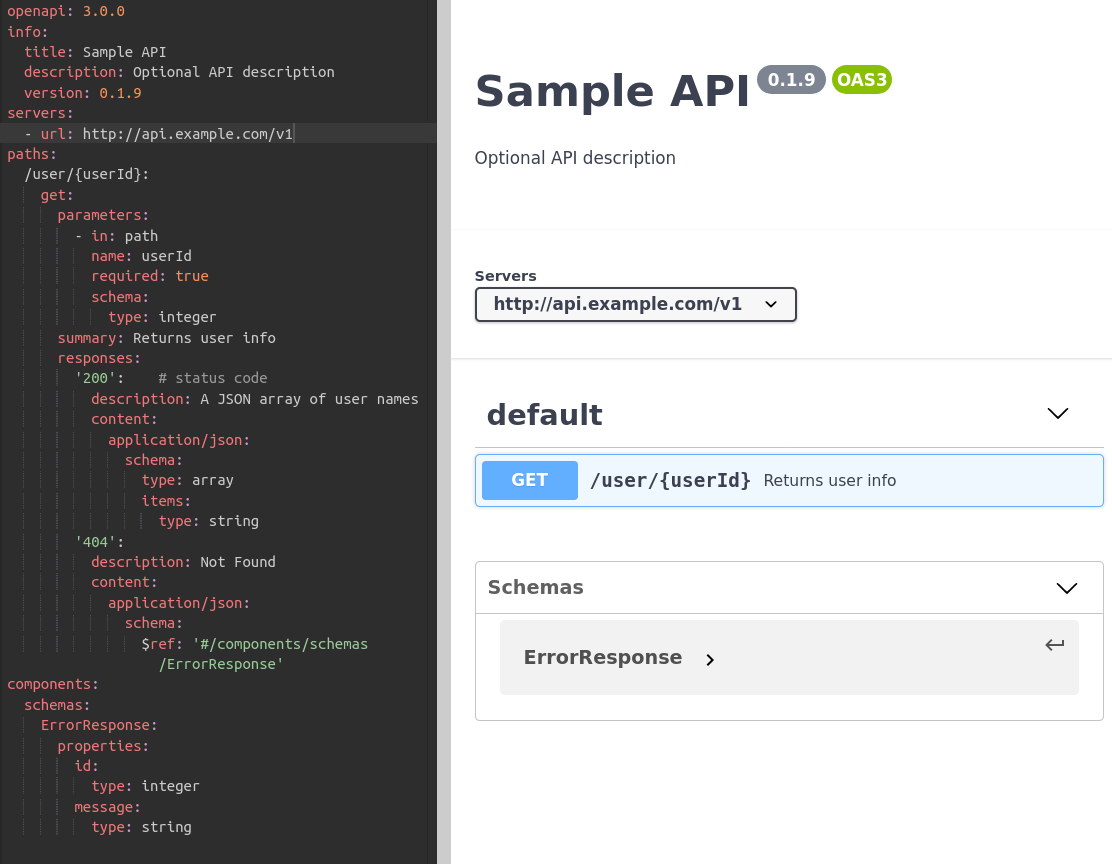
\includegraphics[width=\textwidth]{openapi-specification}
  \caption{OpenAPI specification in YAML format and generated UI}
  \label{fig:openapi-specification}
\end{figure}

Let us have a look at the structure of OpenAPI specification and its separate field to gain a better knowledge about provided information, that can we subseqently use to implement a fuzzer.


% OpenAPI specification, previously known as Swagger, was standardized in 2016 and become overseen by the OpenAPI Initiative \cite{openapi2020main}. The specification describes an API in a machine-readable way (usually in JSON or YAML format). It defines different endpoints of the API along with the required and optional headers and response codes. Besides, it defines the payload fields, types, and encodings. This gives us the advantage of knowing the input structure, thus making it easier to make a \emph{smart} fuzzer.

\subsection{What OpenAPI provides}

\paragraph{}
As we were able to see, OpenAPI specification fully describes the API. Thanks to the specification-provided information we can implement a \emph{smart} fuzzer.
